% !TEX root = main.tex

\section{Introduction}

A dominating set in an undirected and simple graph $G$ is a set
$D\subseteq V(G)$ such that every vertex $v\in V(G)$ either belongs
to $D$ or has a neighbor in $D$.
%The optimization version of the minimum dominating set problem takes as input a graph $G$ and the objective
%is to find a minimum size dominating set of~$G$.
The dominating set problem has many
applications in theory and practice, see e.g.~\cite{du2012connected,sasireka2014applications}, unfortunately
however, already the decision
problem whether a graph admits a dominating set of size $k$
is NP-hard~\cite{karp1972reducibility} and this even holds in
very restricted settings, e.g.\ on planar graphs of maximum degree
$3$~\cite{garey1979computers}.

Consequently, attention
shifted from computing exact solutions to approxi\-mating
near optimal dominating sets. A simple greedy algorithm computes
an $\ln n$ approximation (where $n$ is number of vertices
of the input graph)
of a minimum dominating set \cite{johnson1974approximation,lovasz1975ratio}, and for
general graphs this algorithm is near optimal -- it is NP-hard
to approximate minimum dominating sets within factor
$(1-\epsilon)\ln n$ for every $\epsilon>0$~\cite{dinur2014analytical}.

Therefore, researchers tried to identify restricted
graph classes where better (sequential) approximations are possible.
For example, the problem
admits a PTAS on classes with sub\-exponential expansion~\cite{har2017approximation}. Here, expansion refers to the edge
density of bounded depth minors, which we will define formally
below. Important examples of classes with subexponential
expansion include the class of planar graphs and more generally
classes that exclude some fixed graph as a minor. The dominating
set problem admits a constant factor approximation on classes of
bounded degeneracy (equivalently, of bounded arboricity)~\cite{bansal2017tight,lenzen2010minimum}
and an $\Oof\hspace{1pt}(\ln \gamma)$ approxi\-mation (where~$\gamma$ denotes the size
of a minimum dominating set) on classes of bounded VC-dimension~\cite{bronnimann1995almost,even2005hitting}. In fact, the greedy
algorithm can be modified to yield an $\Oof\hspace{1pt}(\ln \gamma)$
approximation on biclique-free graphs (graphs that exclude some fixed
complete bipartite graph $K_{t,t}$ as a subgraph)~\cite{siebertz2019greedy}
and even a constant factor approximation on
graphs with bounded degeneracy~\cite{jones2017parameterized}.
However, it is unlikely
that polynomial-time constant factor approximations exist even on
$K_{3,3}$-free graphs~\cite{siebertz2019greedy}.
The general goal in this line of research is to identify the broadest
graph classes on which the dominating set problem (or other important
problems that are hard on general graphs) can be approximated
efficiently with a certain guarantee on the approximation factor.
These limits of tractability are often captured by abstract notions, such
as expansion, degeneracy or VC-dimension of graph classes.

\medskip
In this paper we study the distributed time complexity of finding
dominating sets in the classic LOCAL model of distributed computing,
which can be traced back at least to the seminal work of Gallager,
Humblet and Spira~\cite{gallager1983distributed}. In this model, a
distributed system is modeled by an undirected (connected) graph~$G$,
in which every vertex represents a computational entity of the network and every edge represents a bidirectional communication channel. The vertices are equipped with unique identifiers.
In a distributed algorithm, initially, the nodes have no knowledge about
the network graph. They must then communicate and coordinate
their actions by passing messages to one another in order to achieve
a common goal, in our case, to compute a dominating set of the
network graph. The LOCAL model focuses on the aspects of
communication complexity and therefore the main measure for
the efficiency of a distributed algorithm is the number of communication
rounds it needs until it returns its answer.

\medskip
Kuhn et al.~\cite{KuhnMW16} proved that in~$r$ rounds on an~$n$-vertex graphs of maximum degree
$\Delta$ one can approximate minimum dominating sets only within a factor $\Omega(n^{c/r^{\mathrlap{2}}}/r)$
and~$\Omega(\Delta^{1/(r+1)}/r)$, respectively, where~$c$ is a constant.
This implies that, in general, to achieve a constant approximation ratio,
we need at least $\Omega\hspace{1pt}(\sqrt{\log
    n/\log \log n})$ and~$\Omega\hspace{1pt}(\log \Delta/\log \log \Delta)$ communication rounds, respectively.
Kuhn et al.~\cite{KuhnMW16} also presented a~$(1+\epsilon)\ln \Delta$-approximation that runs in $\Oof\hspace{1pt}(\log(n)/\epsilon)$ rounds for any~$\epsilon>0$,
Barenboim et al.~\cite{barenboim2018fast}
presented a deterministic $\Oof\hspace{1pt}((\log n)^{k-1})$-time algorithm that provides an
$\Oof\hspace{1pt}(n^{1/k})$-approximation, for any integer parameter~$k \ge 2$.
More recently, the combined results of Rozhon, Ghaffari, Kuhn, and Maus~\cite{DBLP:conf/stoc/GhaffariKM17,DBLP:conf/stoc/RozhonG20}
provide an algorithm computing a $(1+\epsilon)$-approximation of the dominating set
in poly$(\log(n)/\epsilon)$ rounds~\cite[Corollary 3.11]{DBLP:conf/stoc/RozhonG20}.

Since by the results of Kuhn et al.~\cite{KuhnMW16} in general graphs it is not
possible to compute a constant factor approximation in a constant number
of rounds,
much effort has been invested to improve the ratio between approximation
factor and number of rounds on special graph classes.
For graphs of degeneracy~$a$ (equivalent to arboricity up to factor $2$),
Lenzen and Wattenhofer~\cite{lenzen2010minimum}
provided an algorithm that achieves a factor~$\Oof\hspace{1pt}(a^2)$ approximation
in randomized time~$\Oof\hspace{1pt}(\log n)$, and a deterministic~$\Oof\hspace{1pt}(a \log
\Delta)$ approximation algorithm
with $\Oof\hspace{1pt}(\log \Delta)$ rounds. Graphs of bounded degeneracy include all graphs that exclude a fixed graph as a (topological) minor and in particular, all planar graphs and any class of bounded genus.

Amiri et al.~\cite{akhoondian2018distributed} provided a deterministic
$\Oof\hspace{1pt}(\log n)$ time constant factor approximation algorithm on
classes of bounded expansion (which extends also to connected
dominating sets).
Czygrinow et al.~\cite{czygrinow2008fast} showed
that for any given~\mbox{$\epsilon>0$}, $(1+\epsilon)$-approximations of a maximum independent
set, a maximum matching, and a minimum dominating set, can be computed in
$\Oof\hspace{1pt}(\log^* n)$ rounds in planar graphs, which is asymptotically optimal~\cite{lenzen2008leveraging}.

Lenzen et al.~\cite{lenzen2013distributed} proved that on planar graphs
a 130\hspace{1pt}\raisebox{0.3pt}{-}\hspace{0.9pt}approximation of a minimum dominating set can be computed in a
constant number of
rounds. A careful analysis of Wawrzyniak~\cite{wawrzyniak2014strengthened}
later showed that the algorithm computes in fact a 52\hspace{1pt}\raisebox{0.3pt}{-}\hspace{0.9pt}approximation.
In terms of lower bounds, Hilke et al.~\cite{hilke2014brief} showed that there is no
deterministic local algorithm (constant-time distributed graph algorithm) that
finds a~$(7-\epsilon)$-approximation of a minimum dominating set on
planar graphs, for any positive constant~$\epsilon$. Better approximation
ratios are known for some special cases, e.g.\ 32 if the planar graph is
triangle-free \mbox{\cite[Theorem 2.1]{alipour2020distributed}}, 18 if the planar graph has girth
five~\cite{alipour2020local} and 5 if the graph is
outerplanar (and this bound is tight)~\cite[Theorem 1]{bonamy2021tight}.
Wawrzyniak~\cite{wawrzyniak2013brief} showed
that message sizes of $\mathcal{O}(\log n)$ suffice to give a
constant factor approximation on planar graphs in a constant number
of rounds.

The constant factor approximations in a constant number of rounds for planar
graphs were gradually extended to classes with bounded genus~\cite{akhoondian2016local,amiri2016brief}, classes with sublogarithmic expansion~\cite{amiri2019distributed} and eventually by Czygrinow et al.~\cite{czygrinow2018distributed} to classes with excluded topological minors.
Again, one of the main goals in this line of research is to find the most general
graph classes on which the dominating set problem admits a constant
factor approximation in a constant number of rounds.

\medskip

\begin{figure}[h!]
\begin{center}
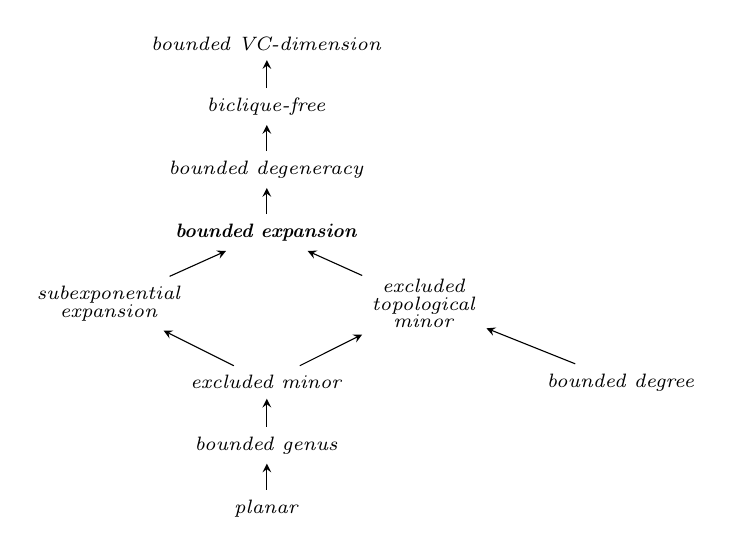
\begin{tikzpicture}

\node (bd-deg) at (11,-2.7) {\scriptsize\textit{bounded degree}};
\node[align=center] (topminor) at (8.5,-1.7) {\scriptsize\textit{excluded}\\[-2mm]\scriptsize\textit{topological}\\[-2mm] \scriptsize\textit{minor}};
\node[align=center] (sublog) at (4.5,-1.7) {\scriptsize\textit{subexponential}\\[-2mm]\scriptsize\textit{expansion}};
\node (bd-exp) at (6.5,-0.8) {\scriptsize\textbf{\textit{bounded expansion}}};
\node (degenerate) at (6.5,0) {\scriptsize\textit{bounded degeneracy}};
\node (biclique-free) at (6.5,0.8) {\scriptsize\textit{biclique-free}};
\node (vc) at (6.5,1.6) {\scriptsize\textit{bounded VC-dimension}};
\node (planar) at (6.5,-4.3) {\scriptsize\textit{planar}};
\node (genus) at (6.5,-3.5) {\scriptsize\textit{bounded genus}};
\node (minor) at (6.5,-2.7) {\scriptsize\textit{excluded minor}};

%%%%%%%%%%%%%%%% Arrows %%%%%%%%%%%%%%%%

\draw[->,>=stealth] (planar) to (genus);
\draw[->,>=stealth] (genus) to (minor);
\draw[->,>=stealth] (minor) to (topminor);
\draw[->,>=stealth] (topminor) to (bd-exp);
\draw[->,>=stealth] (bd-deg) to (topminor);
\draw[->,>=stealth] (minor) to (sublog);
\draw[->,>=stealth] (sublog) to (bd-exp);
%\draw[->,>=stealth] (topminor) to[bend right=10] (bd-exp.east);
\draw[->,>=stealth] (bd-exp) to (degenerate);
\draw[->,>=stealth] (degenerate) to (biclique-free);
\draw[->,>=stealth] (biclique-free) to (vc);

\end{tikzpicture}
\end{center}
\caption{Inclusion diagram of the mentioned graph classes. }
\end{figure}\label{fig:classes}

We take a step towards this goal and generalize the result of
Czygrinow et al.~\cite{czygrinow2018distributed} to classes of bounded
expansion. The notion of bounded expansion was introduced
by Ne\v{s}et\v{r}il and Ossona de Mendez~\cite{nevsetvril2008grad} and
offers an abstract definition of uniform sparseness in graphs. It is based on bounding the density of shallow minors. Intuitively, while
a minor is obtained by contracting arbitrary connected subgraphs of a graph
to single vertices, in an $r$-shallow minor we are only allowed to contract
connected subgraphs of radius at most~$r$.

\medskip
A class of graphs has
bounded expansion if for every radius $r$ the set of all \mbox{$r$-shallow}
minors has edge density bounded by a constant depending only on~$r$.
We write $\nabla_r(G)$ for the maximal edge density of an
$r$-shallow minor of a graph~$G$.
Of course, every class~$\Cc$ that excludes a fixed graph $H$ as
a minor has bounded expansion. For such classes there exists an
absolute constant
$c$ such that for all $G\in\Cc$ and all~$r$
we have $\nabla_r(G)\leq c$.
Special cases are the class of
planar graphs, every class of graphs that can be drawn
with a bounded number of crossings, and every class of graphs
that embeds into a fixed surface.
Every class of intersection graphs of low density objects in low
dimensional Euclidean space has polynomial expansion, that is, the function~$\nabla_r$ is bounded polynomially in $r$ on $\Cc$. Also
every class $\Cc$ that excludes a fixed graph $H$ as
a topological minor has bounded expansion.
Important special cases are classes of
bounded degree and classes of graphs that can be drawn
with a linear number of crossings.
Further examples include
classes of graphs with bounded queue-number, bounded stack-number or bounded
non-repetitive chromatic number. Also, for each constant $d>0$ there is a bounded expansion class $\mathscr R_d$, to which  the Erd\H os-R\'enyi random graphs $G(n,d/n)$ belong
asymptotically almost surely.
See \cite{har2017approximation,nevsetvril2012characterisations} for reference
to  all these examples.

Classes of bounded expansion are more general than
classes excluding a topological minor. However, maybe
not surprisingly, when performing local
computations, it is not properties of minors or topological minors, but
rather of shallow minors that enable the necessary combinatorial arguments
in the algorithms. This observation was already made in the study of the kernelization complexity of dominating set on classes of sparse graphs \cite{DrangeDFKLPPRVS16,eiben2019lossy,EickmeyerGKKPRS17,FabianskiPST19,kreutzer2018polynomial}.
Moreover, bounding the edge density of shallow minors might be needed only up to some depth.
For example, degenerate classes
are those classes where only $\nabla_{\hspace{-1pt}0}(G)$, the edge
density of subgraphs, is bounded, and
these classes are  more general than classes of bounded
expansion.

The algorithm of Czygrinow et al.~\cite{czygrinow2018distributed} for
classes excluding a topological minor is
based on an quite complicated iterative process of choosing dominating
vertices from so called
\emph{pseudo-covers}. Based on the fact that classes excluding a topological minor in particular exclude some complete bipartite graph
$K_{t,t}$ as a subgraph, it is proved that this iterative process terminates
after at most $t$ rounds and
produces a good approximation of a minimum dominating set.

\section{Our contribution}
Our contribution is threefold:
First, we simplify the
arguments used by Czygrinow et al.\ and give a  more accessible
description of their algorithm.
Second, we identify the boundedness of~$\nabla_{\hspace{-1pt}1}(G)$ as the key property that makes the algorithm
work. Classes with only this restriction are less general than degenerate classes, but
 more general than bounded expansion classes.
 We generalize the algorithm to these general classes
 and prove that the pseudo-covering method cannot
be extended further, e.g.\ to classes of bounded degeneracy.
Last, we optimize the bounds that arise in
the algorithm in terms of several parameters.
Czygrinow et al.\ explicitly stated that they did not aim to
optimize any constants, and as presented, the constants in their
construction are enormous.
%
% of $\nabla_{\hspace{-1pt}1}(G)$ (in fact,
%to optimize further, we will later work with the edge density of
%bipartite shallow minors, which we will simply denote by $\nn(G)$).
%\textcolor{red}{We demonstrate
%the improvements in particular in the case of planar graphs. We show
%that the algorithm provides the best known approximation on
%planar graphs. The approximation ratio seems to be
%$2+3\cdot 7+9=33$. The best currently known bounds are $52$.
%This will be bigger because we need the neighborhoods to be
%larger than $k^t(2t+tK)$... Check this.}
%\sebi{If we have not enough time we drop the planar case.}
Even though the constants in our analysis
are still large, they are by magnitudes smaller than those in the
original presentation. The following is our first main theorem.

\begin{theorem}\label{thm:main-general}
Let $\nabla_1>0$ be an integer.
There exists a LOCAL algorithm that computes  in a constant number of rounds, for any input graph $G$ with $\nabla_{\hspace{-1pt}1}(G)\le \nabla_1$, a dominating set
of size~$\mathcal{O}\hspace{1pt}(\gamma(G))$, where
$\gamma(G)$ denotes the size of a minimum dominating set of $G$.
\end{theorem}


Note that the algorithm depends on the constant $\nabla_1$.
The reason for this is that we cannot locally compute or approximate
$\nabla_1(G)$
in a constant number of rounds. This is also
the case for the algorithm of Czygrinow et al., which works with the
assumption that the inputs exclude a complete graph $K_t$ with~$t$~vertices
as a topological minor, a property that can also not be verified locally.
Furthermore, the number of rounds depends on $\nabla_1$.


The algorithm is actually tuned using more parameters, like upper bounds on $\nabla_0(G)$ and
on integers $s$ and $t$ such that the complete bipartite graph $K_{s,t}$
is not subgraph of $G$, in order to  improve the approximation ratio of the algorithm.
However, all these parameters can be upper bounded in terms of $\nabla_1$.
When these parameters are given, the algorithm computes a
$(2(\nabla_0+1)((2\nabla_1)^{4s\nabla_1}+2)\gamma$ approximation
in a number of rounds that depends on $\nabla_1$ and $t$.



%\medskip
%As mentioned above, the method of pseudo-covers cannot be extended
%beyond classes where~$\nabla_{\hspace{-1pt}1}$ is uniformly bounded
%by a constant. Hence, one of the main
%open questions that remains in this line of research is whether we can
%compute constant factor approximations of minimum dominating sets
%in a constant number of rounds in classes of bounded degeneracy, that
%is, classes with uniformly bounded $\nabla_{\hspace{-1pt}0}$.
%Another remaining problem is to further optimize the constants
%in the constructions.

\medskip

Then, we modify and fine-tune the algorithm for graphs
excluding $K_{3,t}$ as a subgraph (and having~$\nabla_1$ bounded).
Important examples of graphs with this property are graphs that
can be embedded into a fixed surface of bounded genus. We prove
the following theorem.

\begin{theorem}\label{thm:K3t-free-total}
Let $\nabla_1>0$ and $t\geq 3$ be integers.
There exists a LOCAL algorithm and a function $C$ that for every
$K_{3,t}$-free graph $G$ with $\nabla_1(G)\leq \nabla_1$ and every
$\epsilon>0$, computes in~$C(\epsilon)$ rounds a dominating
set of size at most $(6\nabla_1+3)\gamma$.
\end{theorem}

Since planar graphs satisfy $\nabla_1\leq 3$ and exclude $K_{3,3}$ as
a subgraph, from \cref{thm:K3t-free-total} we can derive an approximation
factor of $21$ for planar graphs. A more careful analysis leads to the
following theorem.

\begin{theorem}\label{thm:planar}
  There exists a LOCAL algorithm and a function $C$ that for every planar
  input graph~$G$ and $\epsilon>0$, computes in $C(\epsilon)$ rounds a dominating set
  of size at most \mbox{$(11+\e)\cdot\gamma(G)$}.
\end{theorem}

We further analyze our algorithm on restricted classes of planar graphs and
improve the upper bounds in several cases (see \cref{tab:approx_factor}).
%In particular, we tighten the gap between
%the best-known lower bound of~$7$ and the best-known upper
%bound of~$52$ for the approximation ratio on planar graphs,  by showing that the new algorithm
%computes an ($11+\e$)\hspace{1pt}\raisebox{0.3pt}{-}\hspace{0.9pt}approximation on planar graphs.


\begin{table}[h!t]
	\begin{tabular*}{\textwidth}{|c|c|c|c|}
		\hlx{hv}
Graph class&Lower bound&Previous upper bound&Our upper bound\\
\hlx{vhhv}
Planar graphs&\hfill$7-\e$\hfill\cite{hilke2014brief}&\hfill52\hfill\cite{wawrzyniak2014strengthened}&$11+\e$\\
Triangle-free planar graphs&&\hfill$32$\hfill\phantom{5}\cite{alipour2020distributed}&$8+\e$\\
Bipartite planar graphs&&&$7+\e$\\
Outerplanar graphs&\hfill$5$\hfill\phantom{3}\cite{bonamy2021tight}&\hfill$5$\hfill\phantom{5}\cite{bonamy2021tight}&$(8+\e)$\\
Girth $\ge 5$ planar graphs&&\hfill$18$\hfill\phantom{5}\cite{alipour2020local}&$7$\\
\hlx{vh}
	\end{tabular*}
	\caption{Approximation factors for a LOCAL approximation of $\gamma(G)$ is a constant number of rounds. Our algorithm improves the approximation factors in all these cases, except for the class of outerplanar graphs.
	}
	\label{tab:approx_factor}
\end{table}



%, and prove that
%it computes approximations within a factor of ($8+\e$) for triangle-free planar graphs,
%of ($7+\e$) for bipartite planar graphs, of ($8+\e$) for outerplanar graphs, and
%of $7$ for planar graphs of girth~$5$
%(\cref{thm:bip,thm:tri,thm:girth,thm:outer}).
%% We then analyze our algorithm on bipartite planar graphs,
%% triangle-free planar graphs,
%% planar graphs of girth $5$ and outerplanar graphs and prove that
%% it computes a 12, 14, 7 and 12 approximation, respectively (\cref{thm:bip,thm:tri,thm:girth,thm:outer}).
%This
%improves the currently best known approximation ratios of~32
%and~18 for triangle-free planar graphs and planar graphs of girth~$5$,
%respectively, while our algorithm falls short of achieving
%the optimal approximation ratio of~5 on outerplanar graphs.



\medskip
Before we go into the technical details, let us give an overview of the
algorithm. The algorithm works in three phases. Each phase ($i\in \{1,2,3\}$) computes a small set $D_i$ that is added to the output dominating set
(where by a  small set we mean a set whose size is linear in $\gamma$).


The first phase is a preprocessing phase, which was similarly employed in the
algorithm of Lenzen et al.~\cite{lenzen2013distributed}. In a key lemma,
Lenzen et al.\ proved that for planar graphs
there are only few vertices whose open neighborhood
cannot be dominated by at most six vertices. This lemma generalizes
to graphs $G$ where $\nabla_{\hspace{-1pt}1}(G)$ is bounded as
shown in~\cite{amiri2019distributed} (where six is replaced by a different constant depending
on $\nabla_{\hspace{-1pt}1}(G)$). We improve this general lemma and
derive in particular that in the case of planar graphs there are only few
vertices whose open neighborhood cannot be
dominated by \emph{three} other vertices.
We pick these few vertices as the set $D_1$,
remove them from~$G$ and mark all their neighbors as dominated.
Hence, after the first phase the open neighborhoods of all
remaining vertices can be dominated by a constant number of
other vertices.

In the second phase, %in parallel for every vertex $v=v_1$
we compute concurrently for each vertex $v$ all the so-called
\emph{domination sequences} $v_1,\ldots, v_s$ starting at $v$ (see
 \cref{def:dom-sequence} for a formal definition). The analysis of this phase is based
on the construction of
\emph{pseudo-covers} as in the work of Czygrinow et al.~\cite{czygrinow2018distributed} and in the approach of greedy domination
in biclique-free graphs~\cite{siebertz2019greedy}. The domination
sequences intuitively
provide a tool to carry out a fine-grained analysis of the vertices that
can potentially dominate the remaining non-dominated neighborhoods.
All the vertices $v_s$ are gathered in the set~$D_2$ and are removed from $G$, with all their neighbors marked as dominated. For $K_{3,t}$-free graphs, we slightly modify the
algorithm and provide an even finer analysis.

Call  the number  $\dr(v)$ of non-dominated neighbors of a vertex $v$
the \emph{residual degree} of $v$. We prove that
after the second phase we are left with a graph where every vertex
has residual degree at most~$\Dr$ for a constant $\Dr$. In particular, every vertex
from a minimum dominating set of size $\gamma$ can dominate at most $\Dr+1$
non-dominated vertices (each
vertex dominates its neighbors and itself) and we conclude that the set $R$
of non-dominated vertices has size bounded by~$(\Dr+1)\gamma$ . Hence, we could at this
point pick all non-dominated vertices to add at most $(\Dr+1)\gamma$ vertices
and conclude. Instead, we study two different ways to proceed with a third phase.


Our first option for the third phase is to apply an LP-approximation based on
results of Bansal and Umboh~\cite{bansal2017tight}, who showed
that a very simple selection procedure leads to a constant factor
approximation when the solution to the dominating set linear
program (LP) is given. As shown by Kuhn et al.~\cite{kuhn2006price} we can approximate such a solution in a
constant number of rounds when the maximum degree~$\Delta$
of the graph is bounded.
To apply these results, we have to overcome two obstacles. First,
note that even though we have established that the maximum residual
degree is bounded by a constant~$\Dr$, we may still have unbounded maximum
degree~$\Delta$. We overcome this problem by keeping only a few
representative potential dominators around the set $R$ of non-dominated
vertices. By a simple
density argument, there can be only very few high degree vertices left
that we simply select into the dominating set. As a result, we are left with
a graph where $\Delta$ is bounded by a constant. The second obstacle,
which is easily overcome, is that we do not need to dominate the
whole remaining graph but only the set $R$. This requires a small
adaptation of the LP-formulation of the problem and a proof that the
algorithm of Bansal and Umboh still works for this slightly different setting.
In total, in this version of the third phase of the algorithm, we add at most $\Oof(\gamma)$
vertices.
%and in particular, if $G$ is planar at most $(7+\e)\gamma$ vertices to
%the dominating set. This in total leads to a constant factor approximation and
%in the planar case to an $(11+\e)$\hspace{1pt}-\hspace{1pt}approximation.  %(\cref{thm:planar}).


Our second option for the third phase is to design a  distributed version of the
classical greedy algorithm.
We proceed in a greedy manner in $d$ rounds, as follows (where
$d$ is a bound on the maximum residual degree $\Dr$ of the graph after phase 2).
In the first round, if a non-dominated
vertex has a neighbor of residual degree~$d$, it elects one such neighbor into
the dominating set (or if it has residual degree~$d$ itself, it may choose itself).
The neighbors of the chosen elements are
marked as dominated and the residual degrees are updated. Note that
all non-dominated neighbors of a vertex of residual degree~$d$
in this round select a dominator. Hence, the residual degrees
of all vertices of residual degree~$d$ are decreased to~$0$ and, after
this round, there are no vertices of residual degree $d$ left.
In the second round, if a non-dominated vertex has a neighbor
of residual degree~$d-1$, it elects
one such vertex into the dominating set, and so on, until after $d$ rounds
in the final round every vertex selects a dominator. Unlike in the general
case, where
nodes cannot learn the current maximum residual degree in a constant
number of rounds, by establishing
an upper bound on the maximum residual degree and proceeding in exactly
this number of rounds, we ensure that we iteratively exactly selects the
vertices of maximum residual degree. For the case of planar graphs,
we prove that $\Dr\leq 30$. It remains to analyze the performance
of this algorithm.


A simple density argument shows
that there cannot be too many vertices of degree $i\geq 2\nabla_{\hspace{-1pt}0}(G)$ ($i\geq 6$ in a planar graph). At a first glance it seems that the algorithm would perform worst
when in every of the $\dr$ rounds it would pick as many vertices as possible,
as the constructed dominating set would grow as much as possible. However,
this is not the case, as picking many high degree vertices at the same time makes
the largest progress towards dominating the whole graph. It turns
out that there is a delicate balance between the vertices that we pick
in round $i$ and the remaining non-dominated vertices that leads
to the worst case.
%We formulate these conditions as a
%linear program and solve the linear program to obtain our claimed bounds.
For planar graphs in total, this
leads to a 20\hspace{1pt}\raisebox{0.3pt}{-}\hspace{0.9pt}approximation.
While the greedy algorithm falls short of achieving the best approximation
factor, it is much simpler than the LP-based approach, and interesting to
analyze in its own right.

%\bigskip
%\noindent\hrulefill
%\vspace{0mm}
%
%\textit{Acknowledgements.} We thank the anonymous
%referee of the conference submission \cite{heydt2021local}  for pointing
%out that the third phase of our algorithm can be
%improved by the use of LP-based techniques when the maximum
%degree is bounded.

%\medskip
%\textcolor{red}{It may be interesting to discuss also parameterized
%complexity and then provide an fpt algorithm running in $f(\gamma)$
%rounds in the Congest model. In a $K_{t,t}$-free graph find a node
%of locally maximum degree (break ties by ids). Mark its neighbors,
%which helps to find the vertex with largest intersection and iterate.}
